% $Id: template.tex 11 2007-04-03 22:25:53Z jpeltier $

%\documentclass{vgtc}                          % final (conference style)
\documentclass[review]{vgtc}                 % review
%\documentclass[widereview]{vgtc}             % wide-spaced review
%\documentclass[preprint]{vgtc}               % preprint
%\documentclass[electronic]{vgtc}             % electronic version

%% Uncomment one of the lines above depending on where your paper is
%% in the conference process. ``review'' and ``widereview'' are for review
%% submission, ``preprint'' is for pre-publication, and the final version
%% doesn't use a specific qualifier. Further, ``electronic'' includes
%% hyperreferences for more convenient online viewing.

%% Please use one of the ``review'' options in combination with the
%% assigned online id (see below) ONLY if your paper uses a double blind
%% review process. Some conferences, like IEEE Vis and InfoVis, have NOT
%% in the past.

%% Figures should be in CMYK or Grey scale format, otherwise, colour
%% shifting may occur during the printing process.

\let\ifpdf\relax

%% These three lines bring in essential packages: ``mathptmx'' for Type 1
%% typefaces, ``graphicx'' for inclusion of EPS figures. and ``times''
%% for proper handling of the times font family.

\usepackage{mathptmx}
\usepackage{graphicx}
\usepackage{times}

%% We encourage the use of mathptmx for consistent usage of times font
%% throughout the proceedings. However, if you encounter conflicts
%% with other math-related packages, you may want to disable it.

% customer packages
\usepackage{amsmath}
\usepackage{epstopdf}
\usepackage{caption}
\usepackage{subcaption}
\usepackage{multirow}
\usepackage{algorithmicx}
\usepackage{algorithm}
\usepackage{algpseudocode}

%% If you are submitting a paper to a conference for review with a double
%% blind reviewing process, please replace the value ``0'' below with your
%% OnlineID. Otherwise, you may safely leave it at ``0''.
\onlineid{0}

%% declare the category of your paper, only shown in review mode
\vgtccategory{Research}

%% allow for this line if you want the electronic option to work properly
\vgtcinsertpkg

%% In preprint mode you may define your own headline.
%\preprinttext{To appear in an IEEE VGTC sponsored conference.}

%% Paper title.

\title{Probabilistic Streamline Computation using Particle Filtering}

%% This is how authors are specified in the conference style

%% Author and Affiliation (single author).
%%\author{Roy G. Biv\thanks{e-mail: roy.g.biv@aol.com}}
%%\affiliation{\scriptsize Allied Widgets Research}

%% Author and Affiliation (multiple authors with single affiliations).
%%\author{Roy G. Biv\thanks{e-mail: roy.g.biv@aol.com} %
%%\and Ed Grimley\thanks{e-mail:ed.grimley@aol.com} %
%%\and Martha Stewart\thanks{e-mail:martha.stewart@marthastewart.com}}
%%\affiliation{\scriptsize Martha Stewart Enterprises \\ Microsoft Research}

%% Author and Affiliation (multiple authors with multiple affiliations)
\author{Roy G. Biv\thanks{e-mail: roy.g.biv@aol.com}\\ %
        \scriptsize Starbucks Research %
\and Ed Grimley\thanks{e-mail:ed.grimley@aol.com}\\ %
     \scriptsize Grimley Widgets, Inc. %
\and Martha Stewart\thanks{e-mail:martha.stewart@marthastewart.com}\\ %
     \parbox{1.4in}{\scriptsize \centering Martha Stewart Enterprises \\ Microsoft Research}}

%% A teaser figure can be included as follows, but is not recommended since
%% the space is now taken up by a full width abstract.
%\teaser{
%  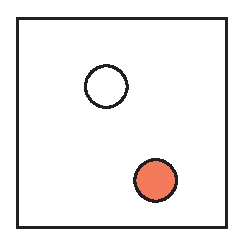
\includegraphics[width=1.5in]{sample.eps}
%  \caption{Lookit! Lookit!}
%}

%% Abstract section.
\abstract{
Streamline-based techniques plays an important role in visualizing and analyzing uncertain steady vector fields. It is a challenging problem to generate accurate streamlines in uncertain vector fields due to the global uncertainty transportation. In this work, we present a novel probabilistic method for streamline computation on distribution-based steady vector fields using a particle filtering framework. In our framework, a streamline is modeled as a state space model which captures the spatial coherence of integration steps and uncertainty in local distributions using the conditional prior density and the likelihood function. To approximate the posterior distribution for all the possible traces originating from a given seed position, a set of weighted samples are iteratively updated from which streamlines with higher likelihood can be derived. We qualitatively and quantitatively compare our method with alternative methods on different types of flow field data sets. Our method can generate possible streamlines with higher certainty and hence more accurate flow traces.
} % end of abstract

% %% ACM Computing Classification System (CCS).
% %% See <http://www.acm.org/class/1998/> for details.
% %% The ``\CCScat'' command takes four arguments.

% \CCScatlist{
%   \CCScat{K.6.1}{Management of Computing and Information Systems}%
% {Project and People Management}{Life Cycle};
%   \CCScat{K.7.m}{The Computing Profession}{Miscellaneous}{Ethics}
% }

%% Copyright space is enabled by default as required by guidelines.
%% It is disabled by the 'review' option or via the following command:
% \nocopyrightspace

%%%%%%%%%%%%%%%%%%%%%%%%%%%%%%%%%%%%%%%%%%%%%%%%%%%%%%%%%%%%%%%%
%%%%%%%%%%%%%%%%%%%%%% START OF THE PAPER %%%%%%%%%%%%%%%%%%%%%%
%%%%%%%%%%%%%%%%%%%%%%%%%%%%%%%%%%%%%%%%%%%%%%%%%%%%%%%%%%%%%%%%%

\begin{document}

%% The ``\maketitle'' command must be the first command after the
%% ``\begin{document}'' command. It prepares and prints the title block.

%% the only exception to this rule is the \firstsection command
\firstsection{Introduction}

\maketitle

%% \section{Introduction}

\section{Related Work}

In this section, we first review previous works related to uncertain flow visualization. Then we give the background and related works about particle filtering.

\textbf{Uncertain Flow Visualization.} One group of the methods focused on visualizing the local uncertainty. This class of algorithms treated uncertainty within the flow field as a local phenomenon. Glyph-based approaches were discussed in~\cite{citeulike:4002316, conf/visualization/LodhaPSW96}, and texture-based methods were proposed in~\cite{botchen:2006:IVUF, 10.1109/VIS.2005.97}. In~\cite{zuk:2008:UBVF}, a method was introduced to visualize uncertainty in bidirectional vector fields. Edge Map was proposed by \cite{10.1109/TVCG.2011.265} to visualize flow fields with quantified spatial and temporal errors. \cite{conf/visualization/SandersonJK04} presented a reaction-diffusion model to visualize the uncertainty. There exist approaches that were designed to visualize global uncertainty which is transported within the flow, such as topology based approaches presented in~\cite{Otto10a, Otto11a}. However, none of the approaches above focused on solving the uncertain particle tracing problem, which is still one of the most popular flow visualization techniques.

\textbf{Particle Filtering.} In this work, we make use of a well-known feature tracking framework called particle filtering~\cite{doucet2001sequential}, which has been successfully used in computer vision and medical image analysis. Many problems in these fields involve tracking unknown quantities from some given observations, such as road tracking and fiber tracking. Generally, prior knowledge has been modeled for these phenomenon and Bayesian models can be formulated with prior distributions for the target of interest and likelihood functions for the observations. Then the tracking problem can be solved based on posterior distributions. The particle filter provides a convenient and attractive approach to evaluate the posterior distributions without any constraint about the data. It has been developed over decades and been successfully applied to solve many real world problems. \cite{bb69534, journals/pami/GemanJ96} applied this approach for human body gestures and road tracking. \cite{Brun02whitematter, bjornemoMICCAI02} introduced particle filtering for probabilistic fiber tracking, which was then improved by~\cite{journals/mia/PontabryROSKD13, Zhang20095}. In visualization community, Zhang et al. also applied this method for tracking the movement of dynamic voxels~\cite{Zhao2012}.


\section{Probabilistic Particle Tracing Model}

In order to analyze the distribution-based flow field by particle tracing, in this section we describe our probability-based particle tracing model.

\subsection{Global Modeling}

Single streamline $L$ originating from position ${x_0}$ can be modeled as $L = \{ {x_0},{x_1},...,{x_n}\} = {x_{0:n}}$, where $x_t$ refers to a position in $\mathrm{R}^d$. As mentioned by Otto et al. in~\cite{Otto10a, Otto11a}, conventional streamline integration methods such as RK4 are not well defined for uncertain vector fields, since there is no unique vector direction at a location ${x_t}$. Therefore, as with most previous methods~\cite{Otto10a, Otto11a}, we make use of the Euler integration model in this paper:
\begin{equation}
  {x_{t + 1}} = {x_t} + {v_t}\Delta t
\end{equation}
where ${v_t}$ and $\Delta t$ refer to the vector direction and the step size at step $t$. If we set the step size $\Delta t$ as a constant, we can represent the streamline by a sequence of vector directions ${L = v_{0:n}}$, since the streamline trajectory only depends on the propagation directions $v_{0:n}$. Figure~\ref{trajectory} depicts an example of the streamline trajectory model.

\begin{figure}[htb]
  \centering
  
\includegraphics[width=2in]{../figures/trajectory.eps}
  \caption{An example streamline generated from a 2D distribution-based vector field is modeled as a sequence of vectors.}
  \label{trajectory}
\end{figure}

For the distribution-based vector fields, there is no unique streamline $v_{0:n}$ for a given starting point $x_0$. Let $\Omega_{x_0}$ be the set of all possible streamlines which originate from $x_0$ given the distribution-based data $\mathcal{H}$, we then can define a probability density function (pdf) over the path space, which is:
\begin{equation}
  p(v_{0:n}|\mathcal{H})
\end{equation}
where $\mathcal{H}$ is the set of observations from the distribution-based data along the streamline trajectory. Here, we denote the distribution obtained at the starting point $x_t$ of a vector $v_t$ as $\lambda_t=\mathcal{H}(v_t)$. By applying the Bayes theorem, the target distribution $p({v_{0:n}}|{\lambda_{0:n}})$ can be represented by the prior density $p({v_{0:n}})$ and the conditional observation density $p({\lambda_{0:n}}|{v_{0:n}})$, as:
\begin{equation}
  p({v_{0:n}}|{\lambda_{0:n}}) = \frac{{p({v_{0:n}})p({\lambda_{0:n}}|{v_{0:n}})}}{{p({\lambda_{0:n}})}}
\end{equation}
where ${p({\lambda_{0:n}})}$ is a normalizing constant for a fixed data realization, which equals to $\int {p({v_{0:n}},{\lambda_{0:n}})} d{v_{0:n}}$.

Scientific simulations commonly represent physical phenomena as continuous functions. Thus, streamlines integrated based on the data generated from such simulations are generically smooth. In the other words, the sequence of vector directions $v_{0:n}$ along the particle trace should transition smoothly when the step size $\Delta t$ is small enough. This constraint can be modeled as a conditional prior density $p({v_t}|{v_{0:t - 1}})$. In this paper, we assume the sequence $v_{0:n}$ forms a Markov chain, which means the vector direction $v_t$ only depends on the previous direction $v_{t-1}$, but not on $v_{t-2},...,v_0$; so:
\begin{equation}
  p({v_t}|{v_{0:t - 1}}) = p({v_t}|{v_{t - 1}})
\end{equation}
where $p({v_t}|{v_{t - 1}})$ denotes the probability density associated with the transition from $v_{t - 1}$ to $v_t$. Hence, the probability density for a given streamline can be formulated as:
\begin{equation}
  p({v_{0:n}}) = p({v_0})\prod\limits_{t = 1}^n {p({v_t}|{v_{t - 1}})}
\end{equation}
where $p(v_0)$ can be defined by a uniform distribution, since no prior knowledge is applied.

By measuring the observations $\lambda_{0:n}$ along a given streamline $v_{0:n}$, we can get the conditional observation density $p({\lambda_{0:n}}|v_{0:n})$, which defines a measure of how the observations match the given path. In the other word, the observation density gives how likely the distributions $\lambda_{0:n}$ will be observed if the given streamline $v_{0:n}$ actually exists in the flow field. Likewise, we assume that the observation measured at a point does not depend on any previous points in the trace, i.e.:
\begin{equation}
  p(\lambda_t|v_{0:t}) = p({\lambda_t}|{v_t})
\end{equation}
which defines the likelihood density:
\begin{equation}
  p({\lambda_{0:n}}|{v_{0:n}}) = \prod\limits_{t = 0}^n {p({\lambda_t}|{v_t})}
\end{equation}

By substituting (5) and (7) into (3), the posterior density $p({v_{0:n}}|{\lambda_{0:n}})$ can be expanded as:
\begin{equation}
  p({v_{0:n}}|{\lambda_{0:n}}) = \frac{{p({v_0})\prod\limits_{t = 1}^n {p({v_t}|{v_{t - 1}})} \prod\limits_{t = 0}^n {p({\lambda_t}|{v_t})} }}{{p({\lambda_{0:n}})}}
\end{equation}

\subsection{Local Modeling}

Based on equation (8), the key components of the posterior density $p({v_{0:n}}|{\lambda_{0:n}})$ are the prior density ${p({v_t}|{v_{t - 1}})}$ and the observation density ${p({\lambda_t}|{v_t})}$. In this section, we will elaborate how to model and estimate these two local densities in detail.

\subsubsection{Prior Density}

Prior density characterizes the relationship between two adjacent vector directions, which prefers to continue in the previous direction and gives decreasing probability for sharper turns. As presented by Zhang et al. in~\cite{Zhang20095}, the von Mises-Fisher distribution~\cite{fisher} has been selected as the prior density due to its mathematical simplicity and tractability. Some other common choices in the literature are the Watson distribution and the Kent distribution.

For a random $d$-dimensional unit vector $v$ on the $(d-1)$-dimensional sphere, with respect to the mean direction $\mu$ and the concentration parameter $\kappa$, the probability density function of the von Mises-Fisher distribution is given by
\begin{equation}
  f_{d}(v| \mu, \kappa)=C_{d}(\kappa)\exp \left( {\kappa \mu^T v } \right)
\end{equation}
where the normalization constant $C_{d}(\kappa)\,$ is
\begin{equation}
  C_{d}(\kappa)=\frac {\kappa^{d/2-1}} {(2\pi)^{d/2}I_{d/2-1}(\kappa)} \,
\end{equation}
in which $I_{d/2-1}$ denotes the modified Bessel function of the first kind and order $d/2-1$.

The parameter $\kappa$ defines in range $\kappa \ge 0$ is used to control the concentration of the distribution around the mean direction $\mu$. The distribution with higher concentration will have a greater $\kappa$ value. For example, the distribution is focused on a point of the sphere defined by $\mu$ for $\kappa  = \infty$, and is uniform on the sphere for $\kappa=0\,$. Figure~\ref{fisher} gives examples of points sampled from 2-dimensional von Mises-Fisher distributions with different $\kappa$.

\begin{figure}[htb!f]
  \centering
  \begin{subfigure}[b]{0.16\textwidth}
    \centering
    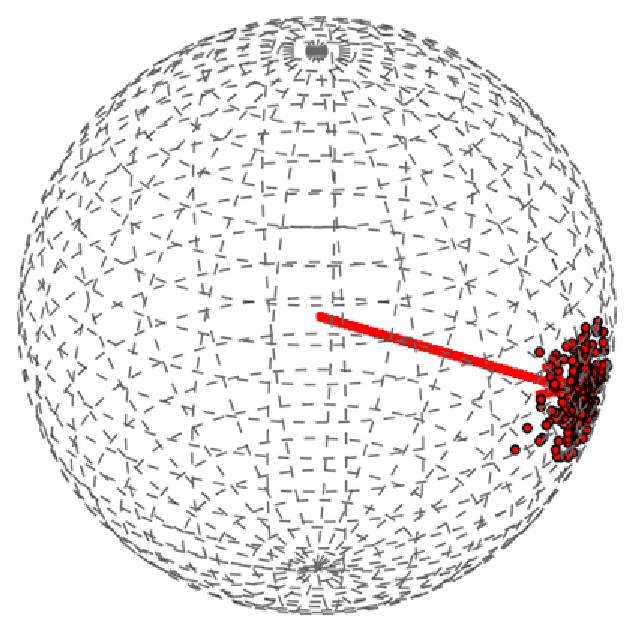
\includegraphics[width=0.9in]{../figures/vf_100.eps}
    \caption{$\kappa=100$}
  \end{subfigure}~
  \begin{subfigure}[b]{0.16\textwidth}
    \centering
    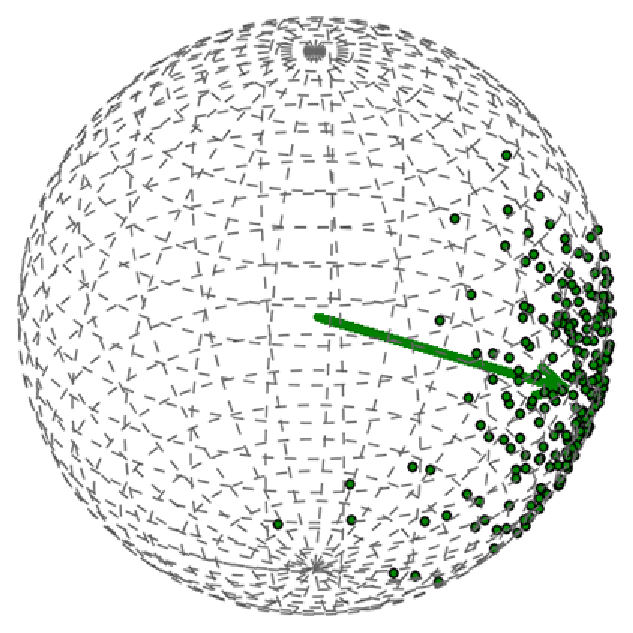
\includegraphics[width=0.9in]{../figures/vf_10.eps}
    \caption{$\kappa=10$}
  \end{subfigure}~
  \begin{subfigure}[b]{0.16\textwidth}
    \centering
    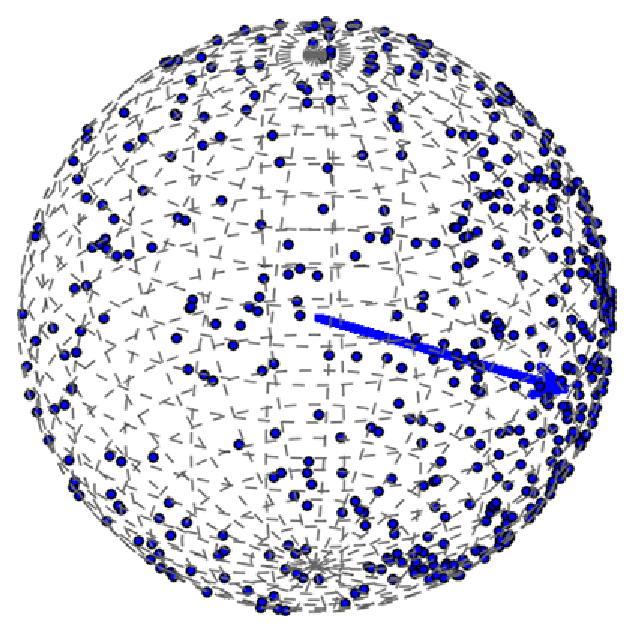
\includegraphics[width=0.9in]{../figures/vf_1.eps}
    \caption{$\kappa=1$}
  \end{subfigure}
  \caption{Points sampled from three von Mises-Fisher distributions on $2$-dimensional spheres with different value of $\kappa$. The mean directions are shown as arrows.}
  \label{fisher}
\end{figure}

In this work, the mean direction $\mu$ of the prior density is given by the previous vector direction ${v_{t - 1}}$. The concentration parameter $\kappa$ is given manually as a constant value. Thus, the prior density $p({v_t}|{v_{t - 1}})$ is defined by the von Mises-Fisher distribution with the mean direction ${v_{t - 1}}$ and the concentration parameter $\kappa$:
\begin{equation}
  p({v_t}|{v_{t - 1}}) = {f_d}({v_t}|{v_{t - 1}}, \kappa)
\end{equation}

\subsubsection{Observation Density}

\section{Stochastic Particle Tracing using Particle Filtering (TODO: update equation numbers.)}

As presented above, the particle tracing result of a given seed position $x_0$ for the distribution-based data $\mathcal{H}$ can be represented as a pdf $p({v_{0:n}}|{\lambda_{0:n}})$ over the trace domain $\Omega_{x_0}$, which is given by equation (8). However, $p({v_{0:n}}|{\lambda_{0:n}})$ is high-dimensional, non-standard, and only known up to a proportionality constant, which makes it infeasible to be evaluated in closed-form. Therefore, a Monte Carlo based method needs to be used to approximate the target distribution. In this work, we make use of the particle filtering technique, which is one of the class of methods known as the Sequential Monte Carlo methods, to estimate the target pdf iteratively.

\subsection{Posterior Approximation with Properly Weighted Traces}

\begin{figure}[htb]
  \centering
  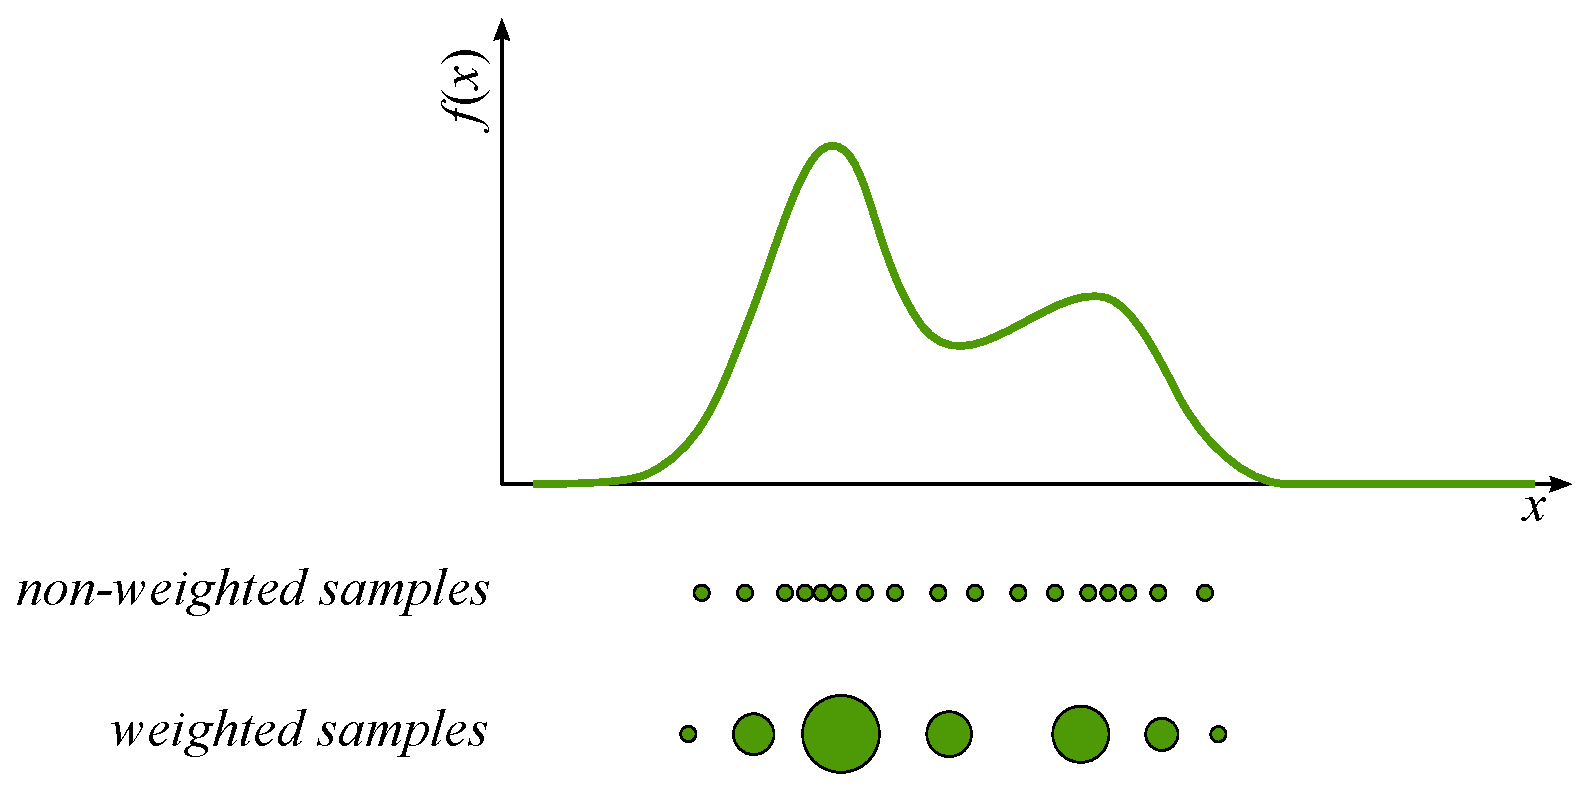
\includegraphics[width=3in]{../figures/importance_sampling.eps}
  \caption{Non-weighted and weighted samples representing the probability density function $f(x)$. Fewer samples is needed to represent the target pdf by using weighted samples.}
  \label{importance_sampling}
\end{figure}

In order to work with the complicated target posterior density $p({v_{0:n}}|{\lambda_{0:n}})$, a more convenient representation is needed to approximate it. By applying the particle filtering method, the target posterior density can be represented by a set of properly weighted traces, which are denoted as $\{ v_{0:n}^i,w_n^i\} _{i = 1}^{{N_s}}$, where $N_s$ is the number of samples and $ w_n^i,i = 0,...,{N_s} $ are the associated weights. Therefore, we can estimate some statistical properties, for example the mean, variance, and maximum likelihood of the target posterior density from the sample traces. Compare to the non-weighted samples used by the conventional Monte Carlo method, weighted samples can represent the target distribution more efficiently. An comparison between weighted and non-weighted samples is illustrated in Figure~\ref{importance_sampling}. A common way of drawing properly weighted samples from the target distribution is to use importance sampling, which samples from an trivial distribution $q({v_{0:n}}|{\lambda_{0:n}})$ called the importance function and assign a weight to each of the random samples according to
\begin{equation}
  w_n = \frac{{p({v_{0:n}}|{\lambda_{0:n}})}}{{q({v_{0:n}}|{\lambda_{0:n}})}}
\end{equation}

\subsection{Sequential Build-Up}

Since the dimension of the target posterior density increases as the number of steps in the particle grows, which makes it difficult to directly obtain the final sample traces with a given step number $n$. By applying particle filtering we smoothly approaching the final probability density by building up the sample traces sequentially with increasing dimensions. To do so, we put ${N_s}$ particles at the seed position $x_0$ and update them iteratively. At each iteration $t$, we have a set of properly weighted samples $\{ v_{0:t-1}^i,w_{t-1}^i\} _{i = 1}^{{N_s}}$ which represents the probability density $p({v_{0:t-1}}|{\lambda_{0:t-1}})$, then each sample can be updated to step $t$ according to the recursive form of the posterior density $p({v_{0:t}}|{\lambda_{0:t}})$, which can be written as:
\begin{equation}
  p({v_{0:t}}|{\lambda_{0:t}}) = p({v_{0:t - 1}}|{\lambda_{0:t - 1}})p(v_t|v_{t-1},\lambda_t)
\end{equation}
where
\begin{equation}
  p(v_t|v_{t-1},\lambda_t) = \frac{{p({\lambda_t}|{v_t})p({v_t}|{v_{t - 1}})}}{{p({\lambda_t}|{\lambda_{0:t - 1}})}}
\end{equation}
Since directly drawing vectors from $p(v_t|v_{t-1},\lambda_t)$ is difficult, we make use of an alternative density function $q({v_t}|{v_{t - 1}},{\lambda_t})$ which is so-call the importance function presented above. From the importance function, vector directions $v_t$ can be obtained, therefore the weights can be updated according to equation (16). Theoretically, the importance function can be any distribution for the vector direction $v_t$. However, a bad choice of the importance function may produce vector directions which have low probability in the target distribution. Hence, the choice of the importance function will influence the performance of the particle filtering algorithm significantly, which will be detailed in the next section. In order to iteratively update the weights on-line, the importance function is chosen to factorize such that:
\begin{equation}
  q({v_{0:t}}|{\lambda_{0:t}}) = q({v_{0:t - 1}}|{\lambda_{0:t - 1}})q({v_t}|{v_{t - 1}},{\lambda_t})
\end{equation}
After getting random vector directions according to the importance density $q({v_t}|{v_{t - 1}},{\lambda_t})$, the weights $\{w_t^i\} _{i = 1}^{{N_s}}$ of traces is updated based on $\{w_{t-1}^i\} _{i = 1}^{{N_s}}$. By substituting (17), (19) into (16), we can get the equation to update the weight:
\begin{equation}
  w_t^i = w_{t - 1}^i\frac{{p({\lambda_t}|v_t^i)p(v_t^i|v_{t - 1}^i)}}{{q(v_t^i|v_{t - 1}^i,{\lambda_t})p({\lambda_t}|{\lambda_{0:t - 1}})}}
\end{equation}
Since the weights can be normalized by:
\begin{equation}
  w_t^i = \frac{{w_t^i}}{{\sum\limits_{j = 1}^{{N_s}} {w_t^j} }}
\end{equation}
the normalizing constant ${p({\lambda_t}|{\lambda_{0:t - 1}})}$ can be ignored. Therefore, the weight update equation can be simplified as
\begin{equation}
  w_t^i \propto w_{t - 1}^i\frac{{p({\lambda_t}|v_t^i)p(v_t^i|v_{t - 1}^i)}}{{q(v_t^i|v_{t - 1}^i,{\lambda_t})}}
\end{equation}

The results provided by the particle filtering algorithm for a given seed position is a set of weighted traces which approximate the posterior probability distribution of the possible traces. We directly render them to see the uncertainty of the particle tracing process. With respect to the goal of visualizing the global phenomenon of the vector fields, streamlines originating from different seed positions need to be visualized together, which make it inappropriate to show all the sample traces for a given seed position all the time. To solve this problem, we extract the trace with highest probability based on the posterior density function and visualize all the optimal traces together. The optimal trace is chosen by maximum a posteriori probability (MAP) estimation, which is the trace with the maximal importance weight.

\subsection{The Degeneracy Problem}

A common issue with the particle filtering algorithm is the degeneracy problem, which is that after several iterations, some samples will have extremely small weights. This means that the contribution of those samples to the posterior distribution is negligible. A reasonable measurement of degeneracy is the effective sample size $N_{eff}$ introduced in~\cite{Liu98sequentialmonte}, which can be estimated by
\begin{equation}
  {N_{eff}} = \frac{1}{{\sum\limits_{i = 1}^{{N_s}} {{{(w_t^i)}^2}} }}
\end{equation}
where $w_t^i$ is the normalized weight. The value of $N_{eff}$ is between $1$ and $N_s$ and the smaller $N_{eff}$ is, the weights degenerate more. The degeneracy problem is an undesirable effect in particle filters. The brute force approach to reduce this effect is to use a very large sample size, which is often impractical. Hence, we focus on two other methods.

\textbf{Resampling} The first method is to perform resampling~\cite{doucet2001sequential, gordon:107} whenever the degeneracy becomes significant (i.e., when $N_{eff}$ is smaller than some hard threshold $N_t$). The key idea of resampling is to remove the traces that have small weights and duplicate the traces which have large weights. To do so, we generate a new set of weighted traces by resampling (with repalcement) $N_s$ times from the given set $\{ v_{0:t}^i,w_t^i\} _{i = 1}^{{N_s}}$, making use of the weights $\{w_t^i\} _{i = 1}^{{N_s}}$ as the probabilities for a sample to be resampled, then reset the weights to $w_t^i = \frac{1}{{{N_s}}}$.

\textbf{Good Choice of Importance Function} The second method is choosing a good importance density $q({v_t}|{v_{t - 1}},{\lambda_t})$. The optimal importance density function that minimizes the variance of the weights $w_t^i$ conditioned on $v_{t-1}$ and $\lambda_t$, pointed out by Doucet et al. in~\cite{Doucet00onsequential}, is $p(v_t|v_{t-1}, \lambda_t)$. However, this optimal importance density requires the evaluation of the integral over the new state, which makes it difficult to sample efficiently from. Hence, we focus on designing a suboptimal importance density which can be easily sampled from and represents $p(v_t|v_{t-1}, \lambda_t)$ well. A usual approach is to use the same distribution as the prior density as the importance function, which is called bootstrap filter or condensation algorithm. However, such importance function may not be always effective, since no observation information is used. As a result, the resulting particles are often outliers of the posterior distribution. Therefore, the observation density is used to determine the $v_t$. Since it is expensive to evaluate the observation density function and there is no need to use the actual observation density as the importance density for the particle filtering method, we choose the observed distribution $\lambda_t$ as the importance density function.

\subsection{Algorithm Summary}

Our stochastic particle tracing algorithm is summarize in Algorithm~\ref{algo:pf}.

\begin{algorithm}[h]
\caption{Streamline Estimation with Particle Filtering} \label{algo:pf}
\begin{algorithmic} [1]

\State Let $x_0$ be a given seed position, $n$ be the number of steps, $N_s$ be the number of samples.
\For {$t=0:n$}
\For {$i=1:N_s$}
\State Sample $v_t^i$ at position $x_t$ according to (14)
\State Compute weight $w_t^i$ according to (13), (14), (15), and (22)
\EndFor
\State Normalize the weights $\{w_t^i\}_{i=1}^{N_s}$ according to (21)
\State Calculate $N_{eff}$ using (23)
\If {$N_{eff} < N_t$}
\State Resample $\{ v_{0:t}^i,w_t^i\} _{i = 1}^{{N_s}}$ to obtain $N_s$ equally-weighted particles $\{ \hat{v}_{0:t}^i,\frac{1}{N_s}\} _{i = 1}^{{N_s}}$
\EndIf
\State Propagate $x_t$ to $x_{t+1}$ according to (1)
\EndFor

\end{algorithmic}
\end{algorithm}


\section{Results and Discussion}

We present results with different types of flow field data sets to evaluate our approach, including synthetic data and spatially aggregated data sets. To demonstrate the effectiveness of the proposed algorithm, we compared it with the Monte Carlo (MC) method, which is the general approach to stochastically trace particles in uncertain flow fields. We performed quantitative comparisons on the resulting streamlines generated by our approach and the MC method with different settings and distance measurements. We also qualitatively compare the most likely streamlines as well as the distributions of possible traces produced by our approach and the MC method by visualizing sample traces on different data sets.

\subsection{Synthetic Data}

We first evaluate the proposed algorithm on the analytical static double-gyre data set proposed by Shadden et al. in~\cite{Shadden2005271}. Gaussian noise is added into the vector field to synthesize the uncertainty. In order to quantitatively evaluate the robustness of the proposed algorithm under the influence of noise, we generate streamlines starting from regularly sampled seed positions for the certain double-gyre data set and use those streamlines as our ground truth. Then, a set of sample traces are generated by the MC method and the Bayesian approach starting from the same seed position presented above for the uncertain double-gyre data set with different noise level, which is controlled by the standard deviation $\sigma$ of the Gaussian noise. All the streamlines were generated with a step size of $0.005$ and a maximum step number of $100$. For the Monte Carlo method and the proposed algorithm, a critical parameter is the number of particles used for each seed. Indeed, more particles will give a more accurate presentation of the target distribution but will take more time to generate the results. Hence, a particle count that balances the accuracy and the computation time need to be studied. Based on~\cite{journals/mia/PontabryROSKD13}, we use $100$ particles for both of the methods in the experiments. To compare the accuracy of the resulting traces, the Hausdorff distance~\cite{Roessl:2012:TVCG} and the Mean of the closest point distance~\cite{Corouge04towardsa} between streamlines were used. Figure~\ref{gerror} gives the average of the distances presented above between the most likely streamlines generated from each method and the ground truth, with increasing $\sigma$ values for the noise in the vector field. The figure reveals that our method can produce most likely traces that are closer to the ground truth and the average of the distances increases more slowly than the MC method as the noise increases.

Besides comparing the accuracy of the most likely traces, it is also important to compare the whole distribution of possible traces generated by each method. We evaluate the accuracy of uncertain streamlines starting from a given seed position by measuring the distance between each individual trace and the ground truth, then we compute the weighted sum of all the distances. For the MC method, all traces are equally weighted. For the proposed method, the weights of the traces described above are used. Figure~\ref{gerror_r} shows that the proposed method can generate more accurate traces with less uncertainty.

\begin{figure}[!htb]
  \centering
  \begin{subfigure}[b]{0.24\textwidth}
    \centering
    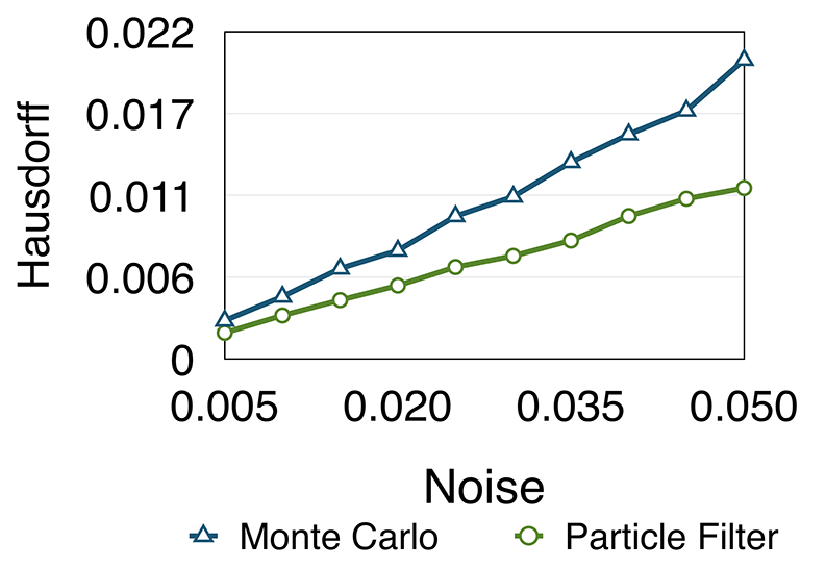
\includegraphics[height=0.8in]{../figures/doublegyre_h.eps}
  \end{subfigure}~
  \begin{subfigure}[b]{0.24\textwidth}
    \centering
    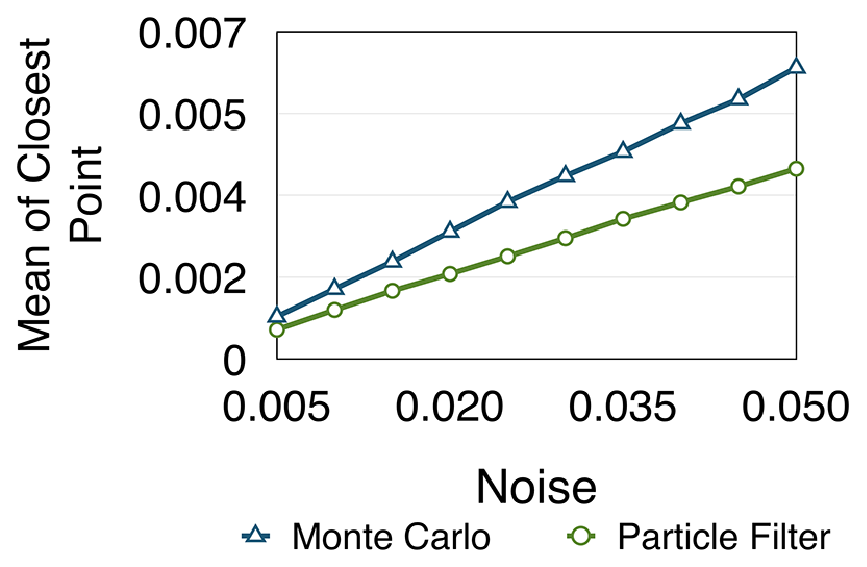
\includegraphics[height=0.8in]{../figures/doublegyre_m.eps}
  \end{subfigure}
  \caption{Comparison of the distance between the most likely traces and the ground truth for our method and the MC method.}
  \label{gerror}
\end{figure}

\begin{figure}[!htb]
  \centering
  \begin{subfigure}[b]{0.24\textwidth}
    \centering
    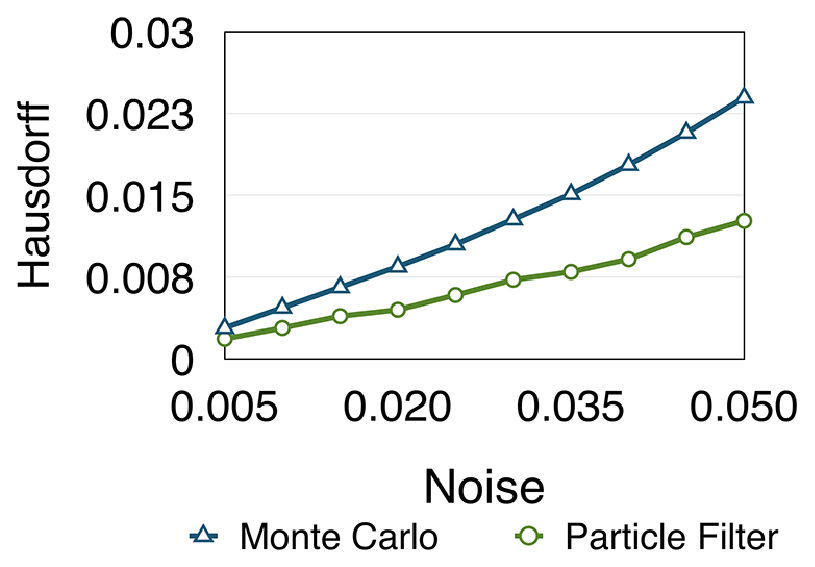
\includegraphics[height=0.8in]{../figures/doublegyre_hr.eps}
  \end{subfigure}~
  \begin{subfigure}[b]{0.24\textwidth}
    \centering
    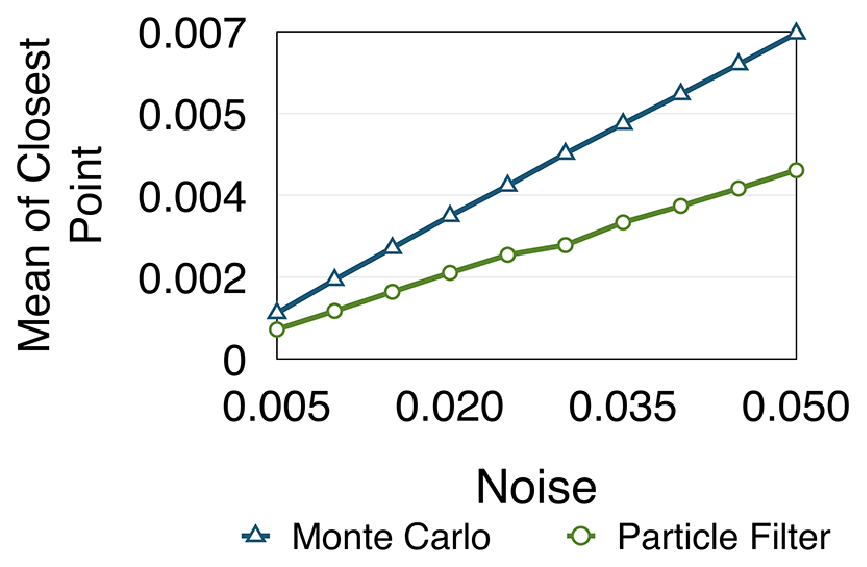
\includegraphics[height=0.8in]{../figures/doublegyre_mr.eps}
  \end{subfigure}
  \caption{Comparison of overall trace accuracy. For each method, distances of all sample traces to the ground truth are measured and summed by their weights.}
  \label{gerror_r}
\end{figure}

Figure~\ref{case_1} shows sample traces generated by the MC method and the proposed method at a given seed location in the double-gyre flow field. As we can see in the figure, our method can generate more concentrated traces which are also closer to the ground truth compared with the MC method. The most likely trace generated by the proposed method is also closer to the ground truth, as shown in~\ref{case_1} (c).

\begin{figure}[!htb]
   \centering
  \small
  (a) \vcenterbox{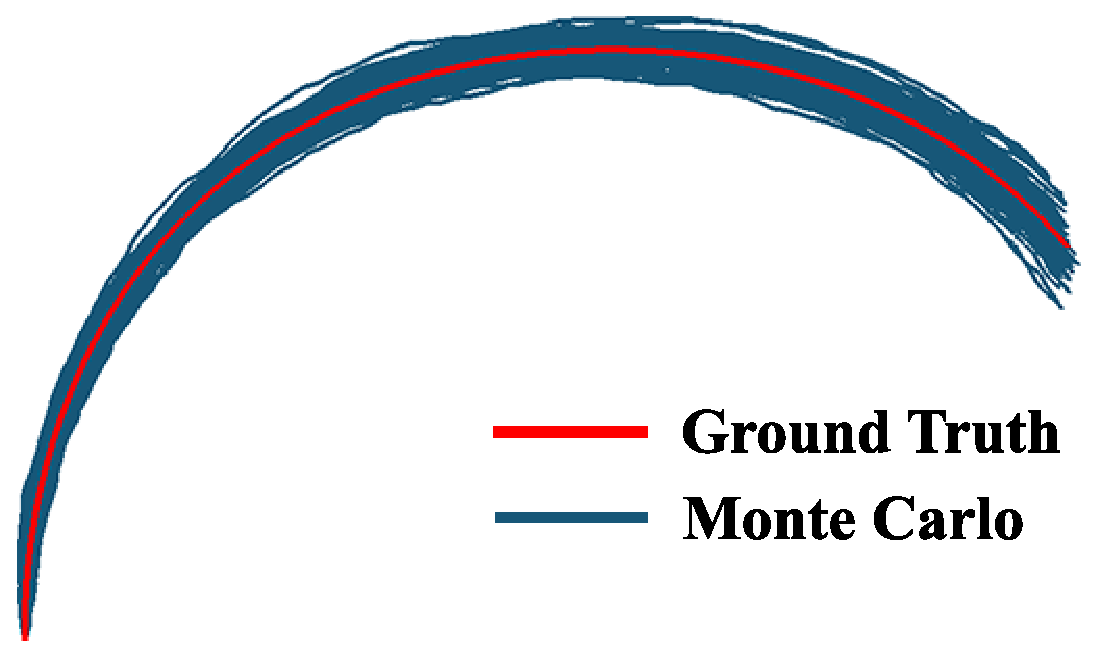
\includegraphics[height=0.5in]{../figures/double_gyre_mc35.eps} } \hfill
  (b) \vcenterbox{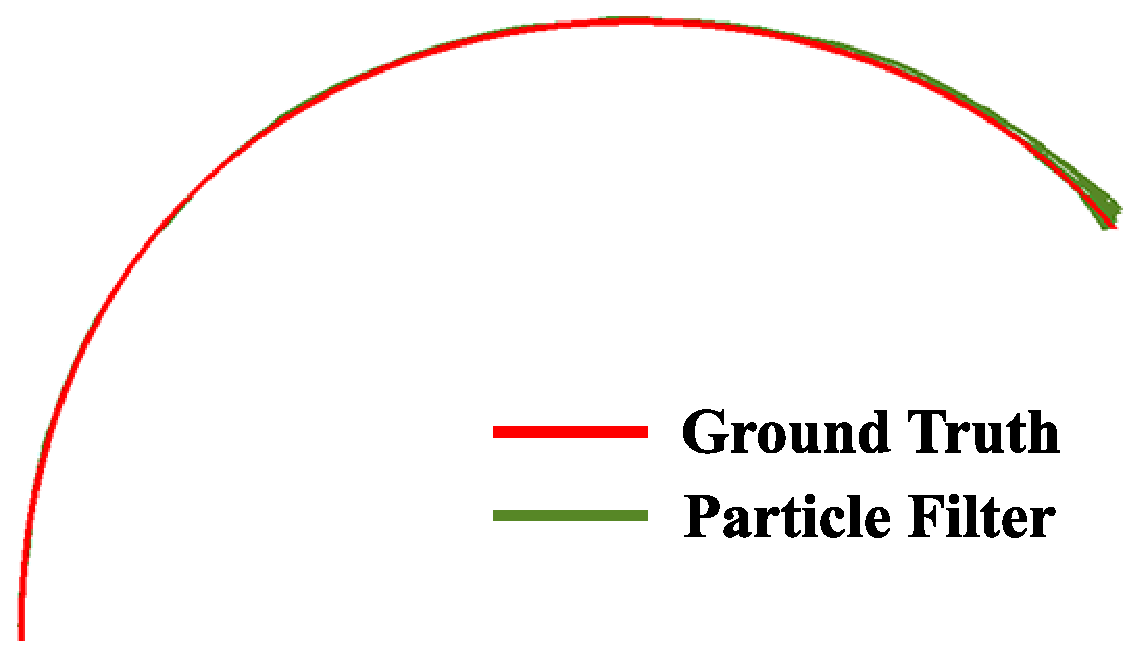
\includegraphics[height=0.5in]{../figures/double_gyre_smc35.eps} } \hfill
  (c) \vcenterbox{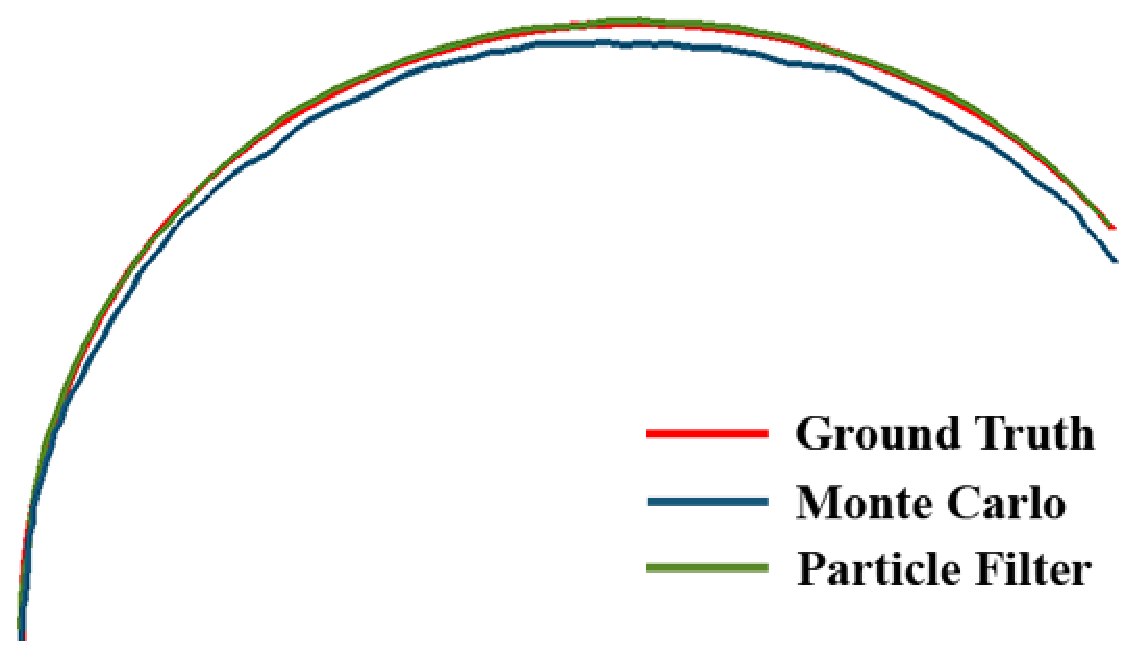
\includegraphics[height=0.5in]{../figures/double_gyre_opt35.eps} }
  \caption{(a): Sampled streamlines computed by the MC method starting from seeding position $x=0.3, y=0.5$ in the analytical double-gyre data set. (b): Sampled streamlines computed by our method from the same seeding position in (a). (c): The most likely traces generated by both methods compared with the ground truth.}
  \label{case_1}
\end{figure}

\subsection{Spatially aggregated Data Sets}

\begin{figure*}[!htbp]
  \centering
  \small
  (a) \vcenterbox{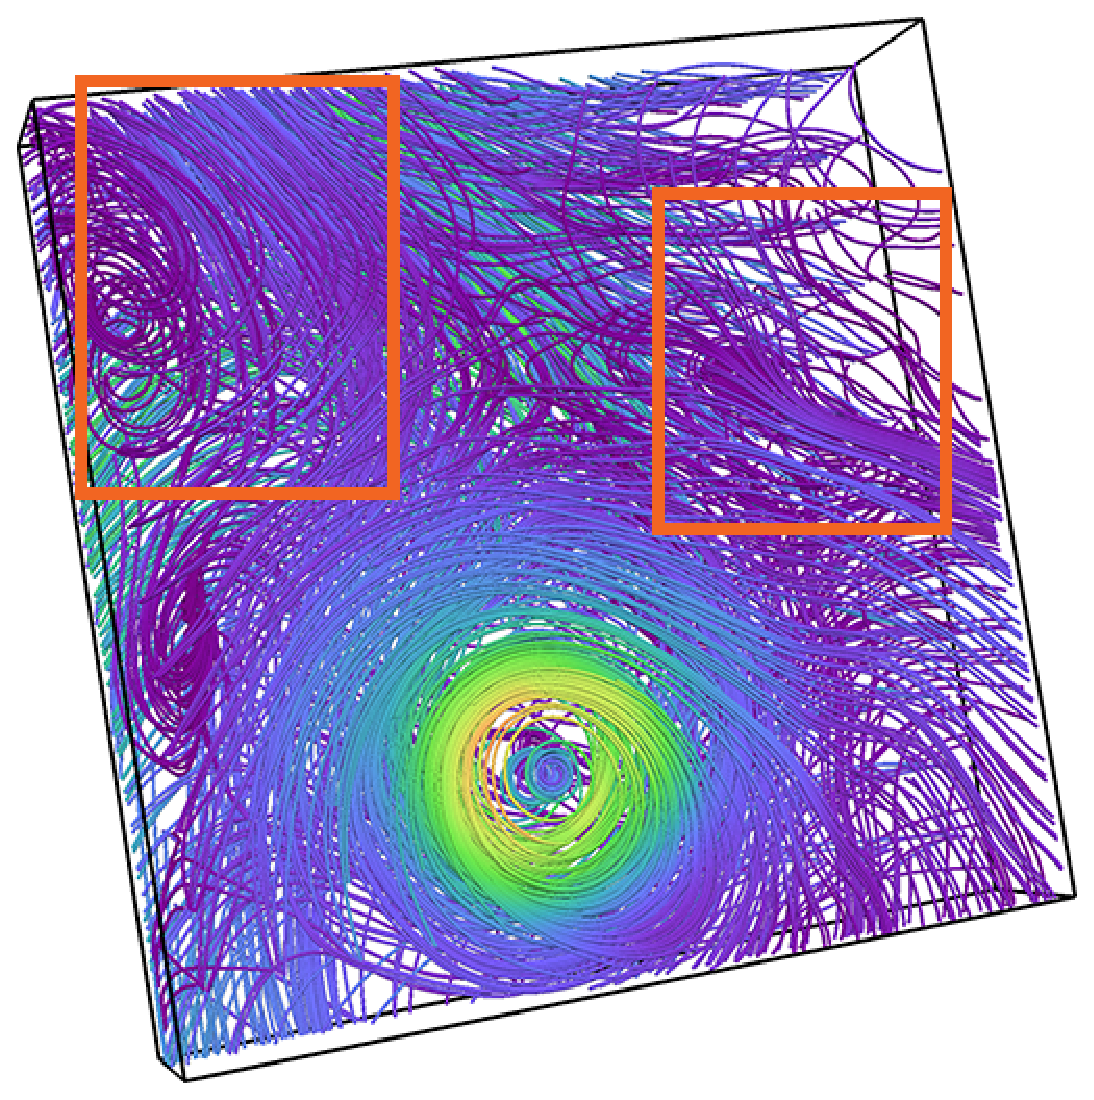
\includegraphics[width=1.5in]{../figures/isabel_gt.eps} } \hfill
  (b) \vcenterbox{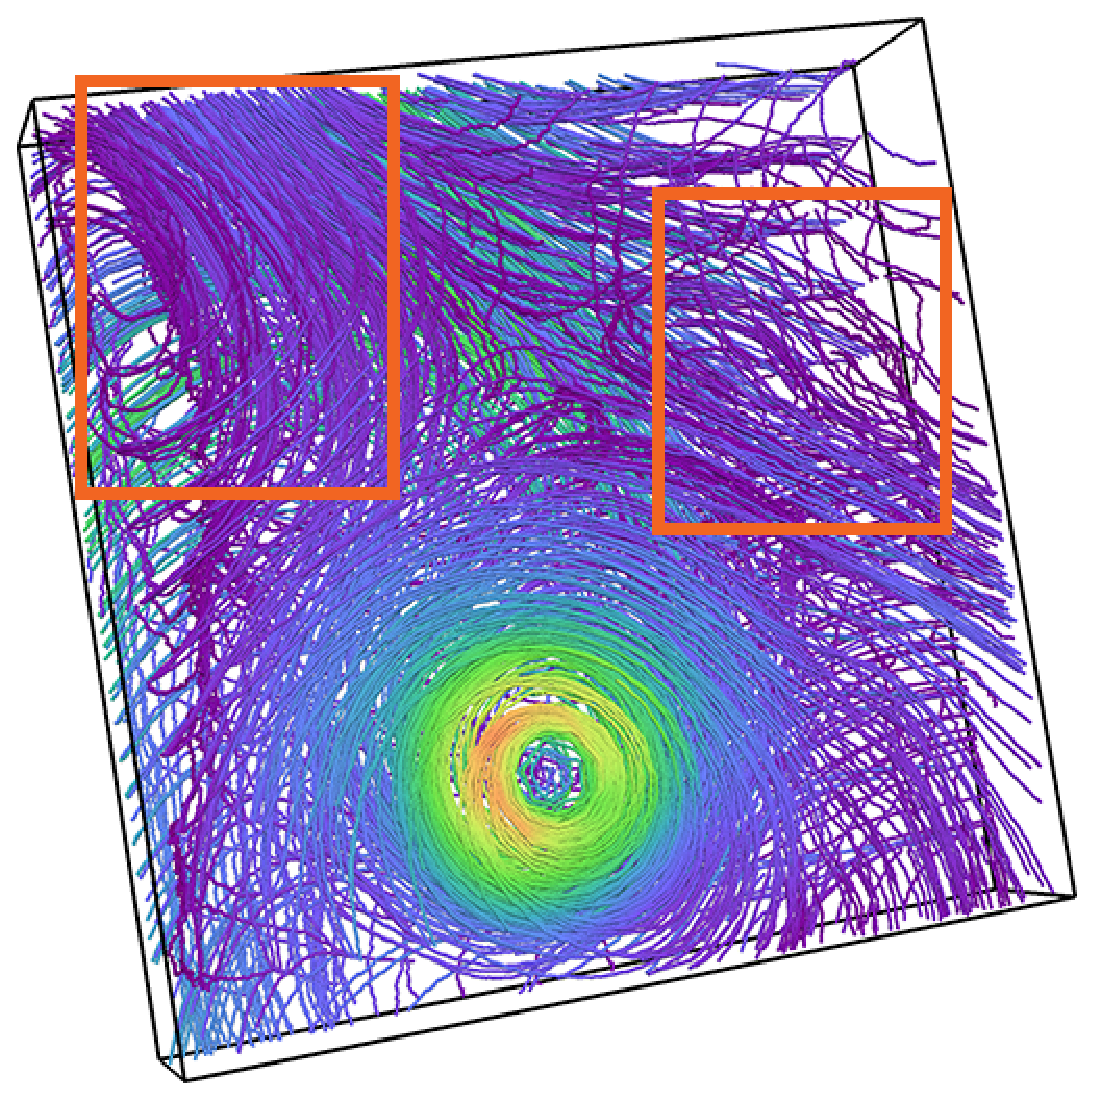
\includegraphics[width=1.5in]{../figures/isabel_mc.eps} } \hfill
  (c) \vcenterbox{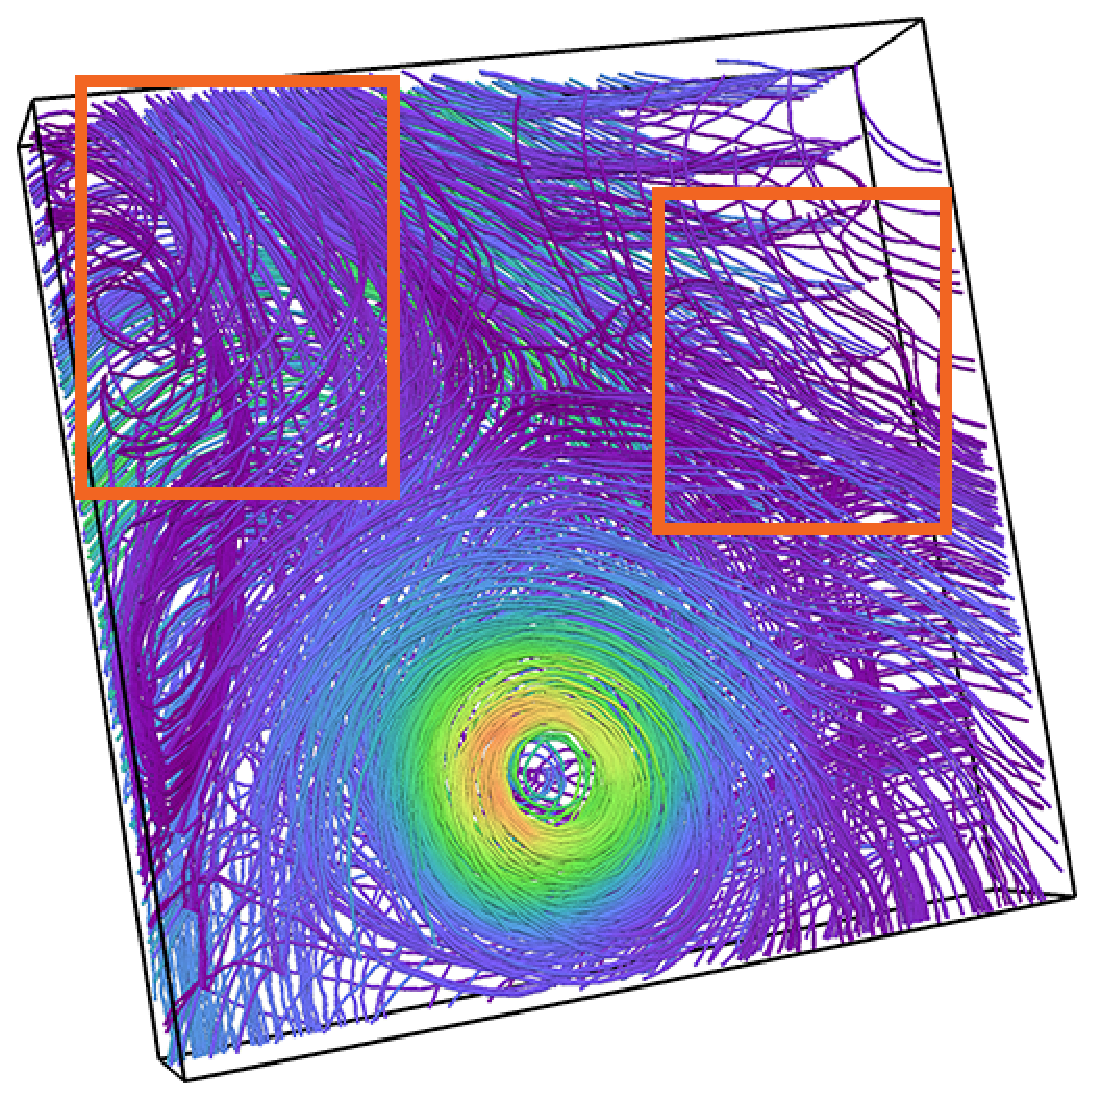
\includegraphics[width=1.5in]{../figures/isabel_smc.eps} }

  \caption{Streamlines generated on the Hurricane Isabel data sets. The color is used to enhance the contrast among streamlines. (a): The ground truth streamlines generated on the raw data. (b): Results produced by the Monte Carlo method on the distribution data with block size $16^3$. (c): Streamlines generated by our method on the same data in (b).}
  \label{data_overview}
\end{figure*}

\begin{figure}[!htbp]
  \centering
  \small
  (a) \vcenterbox{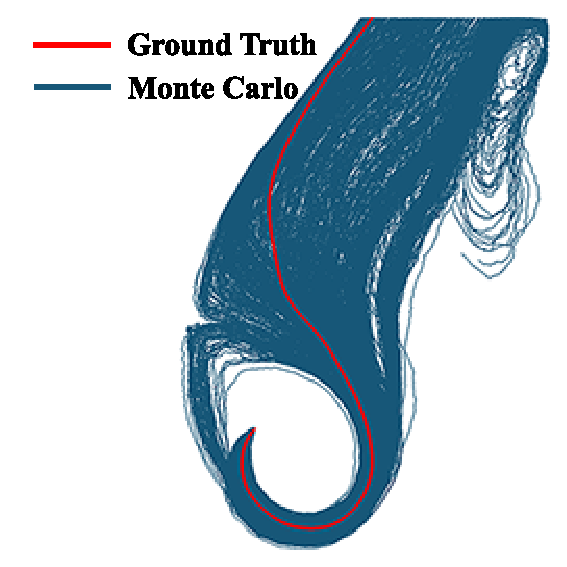
\includegraphics[height=1.0in]{../figures/isabel_mc1.eps} } \hfill
  (b) \vcenterbox{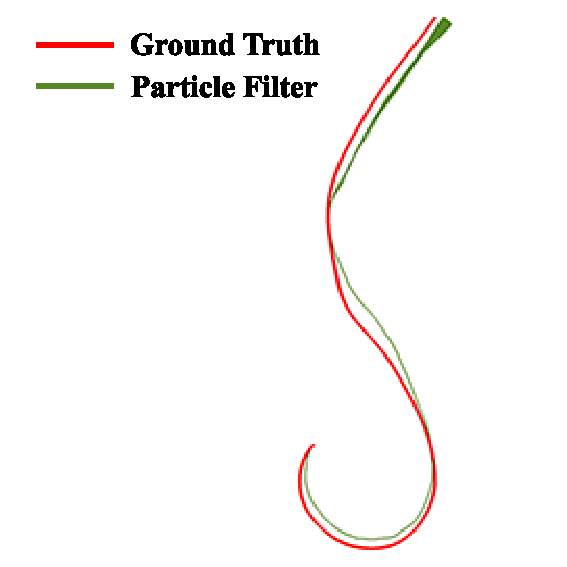
\includegraphics[height=1.0in]{../figures/isabel_smc1.eps} }
  \caption{(a): Sampled streamlines computed by the MC method starting from seeding position $x=250, y=150, z=45$ in the Isabel data set. (b): Sampled streamlines computed by our method from the same seeding position in (a).}
  \label{case_4}
\end{figure}

In this section, experiments were done on the Hurricane Isabel data set. Hurricane Isabel is a data set with a resolution of $500 \times 500 \times 100$ that models a strong hurricane in the west Atlantic region in September 2003. In order to test the performance of our algorithm on uncertain data which represented by non-gaussian distributions, we decompose the data into small cubic blocks and construct a histogram for each block. For the test data set, distribution-based data are generated with three different block size $8^3$, $16^3$, and $32^3$ to evaluate the performance of the proposed algorithm under the influence of uncertainty.

As presented above, we regularly sample a set of seed locations and compute the streamlines for both the raw data and the spatially down sampled data. To perform the quantitative analysis, we treat the streamlines computed from the raw data as the ground truth and compute the distance between the stochastic particle traces with the ground truth. $100$ particles were used with an integration step size $1.0$ and a maximum step number of $1000$ for the streamline computation. Figure~\ref{berror_r} gives the mean of the distances' weighted sum between sample streamline bundles generated from the test methods and the ground truth on the test data set with different block sizes. The figure reveals that the proposed method can produce traces that are closer to the ground truth.

\begin{figure}[!htb]
  \centering
  \begin{subfigure}[b]{0.24\textwidth}
    \centering
    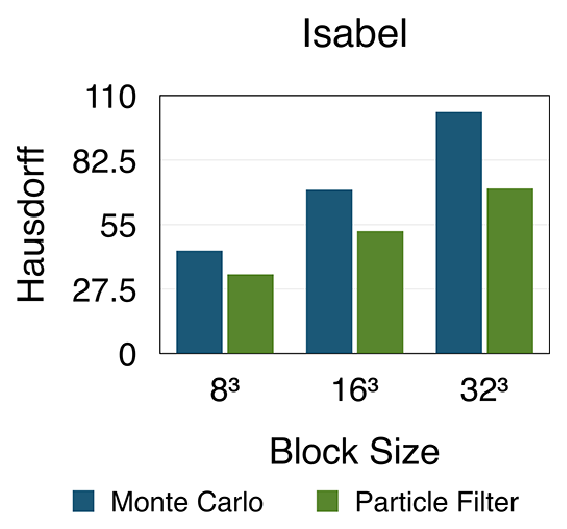
\includegraphics[height=0.9in]{../figures/isabel_h.eps}
  \end{subfigure}~
  \begin{subfigure}[b]{0.24\textwidth}
    \centering
    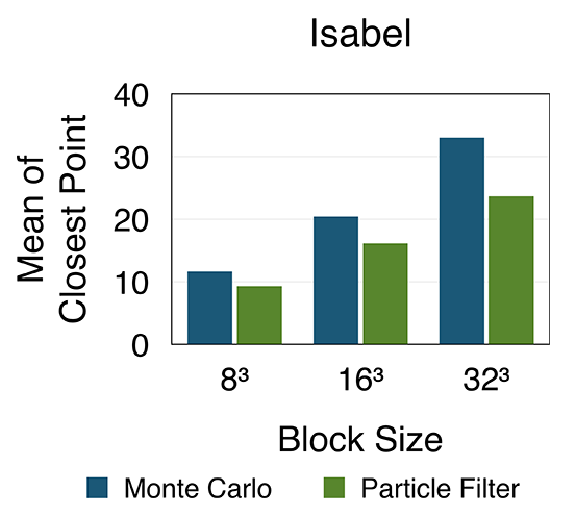
\includegraphics[height=0.9in]{../figures/isabel_m.eps}
  \end{subfigure}
  \caption{Distances between the ground truth and sample traces generated by our method and the MC method for the Isabel data set.}
  \label{berror_r}
\end{figure}

Figure~\ref{data_overview} shows the streamlines generated from the test data set on the seed positions presented above. The most likely streamlines generated by the MC method on the distribution-based data set with block size $16^3$ are given in Figure~\ref{data_overview} (b); as expected, streamlines generated by the MC method are generally not as smooth as the ground truth and some flow features looks quiet different compare with the ground truth. Figure~\ref{data_overview} (c) show the streamlines produced by our method with the same block size, which give more accurate and smoother results. Figure~\ref{case_4} gives sample traces generated by the MC method and the proposed method at a given seed location in the Isabel data set. Figure~\ref{case_4} shows that our algorithm can produce more concentrated and accurate results than the basic MC method, because the correlation between consecutive integration steps are exploited.

\subsection{Performance}

All the experiments were performed on a desktop computer with an Intel(R) Core(TM) i7-4790K CPU 4.0GHz processor, 16GB memory, and an NVIDIA GTX 970 GPU. In Table~\ref{timing}, we compare the performance measurements between the proposed algorithm and the Monte Carlo method for streamlines estimated for a given seed position with $100$ sample points for all the test data sets used in this paper. In all the datasets, our approach is almost as fast as the Monte Carlo method.

\begin{table}[!htb]
\centering
\begin{tabular}{|c|c|c|c|c|}
\hline
\multirow{2}{*}{Data Set}    & \multirow{2}{*}{Method}     & \multicolumn{3}{c|}{Timing(sec)}  \\ \cline{3-5}
                             &                             & 40 Steps  & 80 Steps & 120 Steps  \\ \hline
\multirow{2}{*}{Double Gyre} & MC                          & 0.0026    & 0.005    & 0.008      \\ \cline{2-5}
                             & Bayesian             & 0.0035    & 0.007    & 0.01       \\ \hline
\multirow{2}{*}{Isabel}      & MC                          & 3.3       & 6.7      & 10.1       \\ \cline{2-5}
                             & Bayesian             & 3.4       & 6.8      & 10.7       \\ \hline

\end{tabular}
\caption{Overview of the performance for the proposed algorithm and the Monte Carlo method.}
\label{timing}
\end{table}


\section{Conclusion and Future Work}

In this paper, we present a novel approach for streamline estimation on uncertain steady vector fields. We model the particle tracing problem using a Bayesian framework and solve it using particle filtering. This solution has been tested on two flow field data sets. Compared to the previous methods, our method gives more concentrated traces, and can produce paths of high probability closer to the ground truth.

There are several directions for future research. We will extend our framework to handle time-varying vector datasets, where the specific characteristics of pathlines and streaklines will be taken into account. Secondly, extensions to other flow visualization techniques like FTLE or LIC will be studied.


% %% if specified like this the section will be ommitted in review mode
% \acknowledgements{
% The authors wish to thank A, B, C. This work was supported in part by
% a grant from XYZ.}

\bibliographystyle{abbrv}
%%use following if all content of bibtex file should be shown
%\nocite{*}
\bibliography{draft}
\end{document}
